\section{Простые вычисления}
\subsection{Условие задания}
Выполнить задание. Номер варианта --- 8.

Выражение:
\begin{equation}
\frac{\cos{2x^2} + \sin^2{y}}{x + y} + yx
\end{equation}

Проверить работу созданного приложения на приведенных тестовых примерах. Тесты сделаны на Visual Studio 2008, поэтому обращайте внимание только на первые шесть цифр после запятой.

Приложение должно содержать следующие компоненты:

\begin{enumerate}
\item Заголовок формы должен отражать суть задания.
\item Все элементы формы должны быть внятно подписаны (кнопки подписаны, у тестового поля должно быть написано, для чего оно нужно и т. д.)
\item В коде должны быть комментарии и отступы (код должен быть легко читаем).
\item Должна быть проверка ошибок - ввод не числа, ввод числа, находящегося за пределами ОДЗ, ввод числа, принадлежащего ОДЗ.
\item Если надо ввести 2 значения, то в случае ввод букв в оба поля, ошибка должна быть у обоих полей; в случае ввода одной буквы - только у того поля, где буква.
\end{enumerate}

\subsection{Основы тригонометрии}
В Евклидовой геометрии синусом угла называют отношение противолежащего этому углу катета к гипотенузе. Косинус угла --- отношение прилежащего к этому углу катета к гипотенузе.

Математический анализ обобщает эти функции на всю числовую прямую, делая их периодическими с периодом $2\pi$.

Таким образом $\forall x \in \mathbb{R}\; \exists \sin{x}, \cos{x} \in \mathbb{R}$.

\subsection{Нахождение значений функций синуса и косинуса}
Для нахождения значений выражений мы воспользуемся встроенной в C++ библиотекой cmath.

\subsection{Вид формы в конструкторе}
Форма имеет вид:

\begin{figure}
\centering
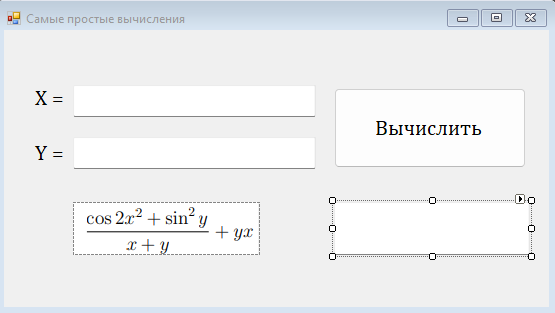
\includegraphics[width=0.5\linewidth]{images/simple-calculations/form.png}
\caption{Форма окна для задания <<Простые вычисления>>}
\label{simple-calculations-form}
\end{figure}

\subsection{Таблица с описанием элементов формы}
Все элементы формы были переименованы для большей читаемости. В таблице \ref{tab:simple-calculations-form} представлены все изменения.

\begin{table}
\centering
\begin{tabular}{|m{0.3\textwidth}|m{0.3\textwidth}|m{0.3\textwidth}|}
\hline
\textbf{Описание элементов формы} & \textbf{Список изменённых атрибутов} & \textbf{Новое значение атрибута} \\
\hline
\hline
Окно формы & Text & Самые простые вычисления \\
Метка для X & Name & xLabel\\
Метка для Y & Name & yLabel \\
Поле для ввода X & Name & xTextbox \\
Поле для ввода Y & Name & yTextbox \\
Поле для вывода & Name & outputTextbox \\
Поле для выражения PictureBox & Name & expressionPicturebox \\
Кнопка <<Вычислить>> & Name & calculateButton \\
\hline
\end{tabular}
\caption{Значение атрибутов элементов в приложении для простых вычислений}
\label{tab:simple-calculations-form}
\end{table}

\subsection{Примеры правильной и неправильной работы приложения}
При запуске приложения на экране появляется окно \ref{fig:simple-calculations-start}.

\begin{figure}
\centering
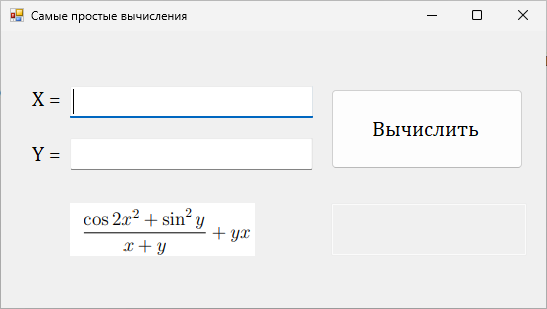
\includegraphics[width=0.5\linewidth]{images//simple-calculations/start.png}
\caption{Запуск программы}
\label{fig:simple-calculations-start}
\end{figure}

При нажатии на кнопку подсчитывается и подставляется значение в поле вывода. Также происходит обработка ошибок.

\begin{figure}
\centering
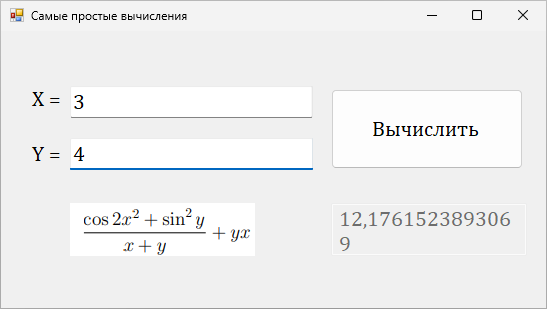
\includegraphics[width=0.5\linewidth]{images//simple-calculations/okay.png}
\caption{Запуск с корректными данными}
\label{fig:simple-calculations-okay}
\end{figure}

\begin{figure}
\centering
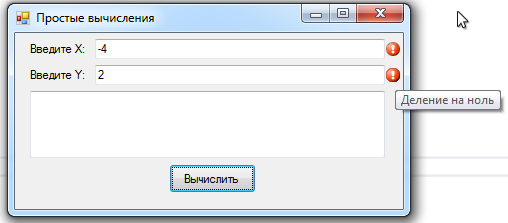
\includegraphics[width=0.5\linewidth]{images//simple-calculations/error.png}
\caption{Пример ввода с программно корректными, но математически некорректными данными}
\label{fig:simple-calculations-error}
\end{figure}

\begin{figure}
\centering
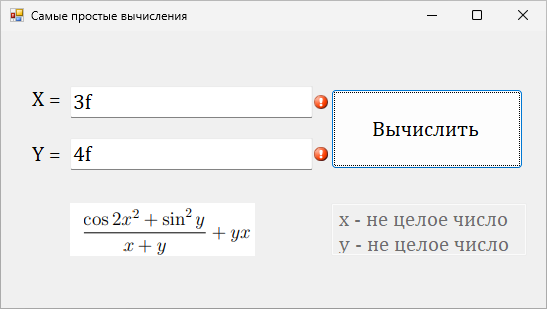
\includegraphics[width=0.5\linewidth]{images//simple-calculations/error2.png}
\caption{Пример ввода с программно некорректными данными}
\label{fig:simple-calculations-error2}
\end{figure}

\subsection{Примеры исходного кода}
\begin{minted}{cpp}
	/* обработка события нажатия на кнопку вычисления */
	private: System::Void btnCalculate_Click(System::Object^ sender, System::EventArgs^ e) {
		ClearAll();
		long long InputX;
		long long InputY;
		// переводим сторку из TextBox в число
		bool parseX = Int64::TryParse(this->inputX->Text, InputX);
		bool parseY = Int64::TryParse(this->inputY->Text, InputY);
		// ввели не число
		if (!parseX) {
			errorProviderX->SetError(inputX, "Введено не целое число");
			if (!parseY) {
				errorProviderY->SetError(inputY, "Введено не целое число");
			}
		}
		else if (!parseY) {
			errorProviderY->SetError(inputY, "Введено не целое число");
		}
		// проверка на деление на ноль
		else {
			if ((InputX == 0 && InputY == 0) || 
				(InputX == -4 && abs(InputY) == 2)) {
				errorProviderX->SetError(inputX, "Деление на ноль");
				errorProviderY->SetError(inputY, "Деление на ноль");
			}
			else{
				double resOutput = solve(InputX, InputY);
				this->output->Text = System::Convert::ToString(resOutput);
			}
		}
	}
\end{minted}

Больше кода проекта доступно в приложении \ref{application-A}. Также в приложенном архиве можно найти полный код проекта.